% Options for packages loaded elsewhere
\PassOptionsToPackage{unicode}{hyperref}
\PassOptionsToPackage{hyphens}{url}
\PassOptionsToPackage{dvipsnames,svgnames,x11names}{xcolor}
%
\documentclass[
]{article}

\usepackage{amsmath,amssymb}
\usepackage{iftex}
\ifPDFTeX
  \usepackage[T1]{fontenc}
  \usepackage[utf8]{inputenc}
  \usepackage{textcomp} % provide euro and other symbols
\else % if luatex or xetex
  \usepackage{unicode-math}
  \defaultfontfeatures{Scale=MatchLowercase}
  \defaultfontfeatures[\rmfamily]{Ligatures=TeX,Scale=1}
\fi
\usepackage{lmodern}
\ifPDFTeX\else  
    % xetex/luatex font selection
\fi
% Use upquote if available, for straight quotes in verbatim environments
\IfFileExists{upquote.sty}{\usepackage{upquote}}{}
\IfFileExists{microtype.sty}{% use microtype if available
  \usepackage[]{microtype}
  \UseMicrotypeSet[protrusion]{basicmath} % disable protrusion for tt fonts
}{}
\makeatletter
\@ifundefined{KOMAClassName}{% if non-KOMA class
  \IfFileExists{parskip.sty}{%
    \usepackage{parskip}
  }{% else
    \setlength{\parindent}{0pt}
    \setlength{\parskip}{6pt plus 2pt minus 1pt}}
}{% if KOMA class
  \KOMAoptions{parskip=half}}
\makeatother
\usepackage{xcolor}
\setlength{\emergencystretch}{3em} % prevent overfull lines
\setcounter{secnumdepth}{5}
% Make \paragraph and \subparagraph free-standing
\makeatletter
\ifx\paragraph\undefined\else
  \let\oldparagraph\paragraph
  \renewcommand{\paragraph}{
    \@ifstar
      \xxxParagraphStar
      \xxxParagraphNoStar
  }
  \newcommand{\xxxParagraphStar}[1]{\oldparagraph*{#1}\mbox{}}
  \newcommand{\xxxParagraphNoStar}[1]{\oldparagraph{#1}\mbox{}}
\fi
\ifx\subparagraph\undefined\else
  \let\oldsubparagraph\subparagraph
  \renewcommand{\subparagraph}{
    \@ifstar
      \xxxSubParagraphStar
      \xxxSubParagraphNoStar
  }
  \newcommand{\xxxSubParagraphStar}[1]{\oldsubparagraph*{#1}\mbox{}}
  \newcommand{\xxxSubParagraphNoStar}[1]{\oldsubparagraph{#1}\mbox{}}
\fi
\makeatother

\usepackage{color}
\usepackage{fancyvrb}
\newcommand{\VerbBar}{|}
\newcommand{\VERB}{\Verb[commandchars=\\\{\}]}
\DefineVerbatimEnvironment{Highlighting}{Verbatim}{commandchars=\\\{\}}
% Add ',fontsize=\small' for more characters per line
\usepackage{framed}
\definecolor{shadecolor}{RGB}{241,243,245}
\newenvironment{Shaded}{\begin{snugshade}}{\end{snugshade}}
\newcommand{\AlertTok}[1]{\textcolor[rgb]{0.68,0.00,0.00}{#1}}
\newcommand{\AnnotationTok}[1]{\textcolor[rgb]{0.37,0.37,0.37}{#1}}
\newcommand{\AttributeTok}[1]{\textcolor[rgb]{0.40,0.45,0.13}{#1}}
\newcommand{\BaseNTok}[1]{\textcolor[rgb]{0.68,0.00,0.00}{#1}}
\newcommand{\BuiltInTok}[1]{\textcolor[rgb]{0.00,0.23,0.31}{#1}}
\newcommand{\CharTok}[1]{\textcolor[rgb]{0.13,0.47,0.30}{#1}}
\newcommand{\CommentTok}[1]{\textcolor[rgb]{0.37,0.37,0.37}{#1}}
\newcommand{\CommentVarTok}[1]{\textcolor[rgb]{0.37,0.37,0.37}{\textit{#1}}}
\newcommand{\ConstantTok}[1]{\textcolor[rgb]{0.56,0.35,0.01}{#1}}
\newcommand{\ControlFlowTok}[1]{\textcolor[rgb]{0.00,0.23,0.31}{\textbf{#1}}}
\newcommand{\DataTypeTok}[1]{\textcolor[rgb]{0.68,0.00,0.00}{#1}}
\newcommand{\DecValTok}[1]{\textcolor[rgb]{0.68,0.00,0.00}{#1}}
\newcommand{\DocumentationTok}[1]{\textcolor[rgb]{0.37,0.37,0.37}{\textit{#1}}}
\newcommand{\ErrorTok}[1]{\textcolor[rgb]{0.68,0.00,0.00}{#1}}
\newcommand{\ExtensionTok}[1]{\textcolor[rgb]{0.00,0.23,0.31}{#1}}
\newcommand{\FloatTok}[1]{\textcolor[rgb]{0.68,0.00,0.00}{#1}}
\newcommand{\FunctionTok}[1]{\textcolor[rgb]{0.28,0.35,0.67}{#1}}
\newcommand{\ImportTok}[1]{\textcolor[rgb]{0.00,0.46,0.62}{#1}}
\newcommand{\InformationTok}[1]{\textcolor[rgb]{0.37,0.37,0.37}{#1}}
\newcommand{\KeywordTok}[1]{\textcolor[rgb]{0.00,0.23,0.31}{\textbf{#1}}}
\newcommand{\NormalTok}[1]{\textcolor[rgb]{0.00,0.23,0.31}{#1}}
\newcommand{\OperatorTok}[1]{\textcolor[rgb]{0.37,0.37,0.37}{#1}}
\newcommand{\OtherTok}[1]{\textcolor[rgb]{0.00,0.23,0.31}{#1}}
\newcommand{\PreprocessorTok}[1]{\textcolor[rgb]{0.68,0.00,0.00}{#1}}
\newcommand{\RegionMarkerTok}[1]{\textcolor[rgb]{0.00,0.23,0.31}{#1}}
\newcommand{\SpecialCharTok}[1]{\textcolor[rgb]{0.37,0.37,0.37}{#1}}
\newcommand{\SpecialStringTok}[1]{\textcolor[rgb]{0.13,0.47,0.30}{#1}}
\newcommand{\StringTok}[1]{\textcolor[rgb]{0.13,0.47,0.30}{#1}}
\newcommand{\VariableTok}[1]{\textcolor[rgb]{0.07,0.07,0.07}{#1}}
\newcommand{\VerbatimStringTok}[1]{\textcolor[rgb]{0.13,0.47,0.30}{#1}}
\newcommand{\WarningTok}[1]{\textcolor[rgb]{0.37,0.37,0.37}{\textit{#1}}}

\providecommand{\tightlist}{%
  \setlength{\itemsep}{0pt}\setlength{\parskip}{0pt}}\usepackage{longtable,booktabs,array}
\usepackage{calc} % for calculating minipage widths
% Correct order of tables after \paragraph or \subparagraph
\usepackage{etoolbox}
\makeatletter
\patchcmd\longtable{\par}{\if@noskipsec\mbox{}\fi\par}{}{}
\makeatother
% Allow footnotes in longtable head/foot
\IfFileExists{footnotehyper.sty}{\usepackage{footnotehyper}}{\usepackage{footnote}}
\makesavenoteenv{longtable}
\usepackage{graphicx}
\makeatletter
\newsavebox\pandoc@box
\newcommand*\pandocbounded[1]{% scales image to fit in text height/width
  \sbox\pandoc@box{#1}%
  \Gscale@div\@tempa{\textheight}{\dimexpr\ht\pandoc@box+\dp\pandoc@box\relax}%
  \Gscale@div\@tempb{\linewidth}{\wd\pandoc@box}%
  \ifdim\@tempb\p@<\@tempa\p@\let\@tempa\@tempb\fi% select the smaller of both
  \ifdim\@tempa\p@<\p@\scalebox{\@tempa}{\usebox\pandoc@box}%
  \else\usebox{\pandoc@box}%
  \fi%
}
% Set default figure placement to htbp
\def\fps@figure{htbp}
\makeatother

\usepackage{booktabs}
\usepackage{longtable}
\usepackage{array}
\usepackage{multirow}
\usepackage{wrapfig}
\usepackage{float}
\usepackage{colortbl}
\usepackage{pdflscape}
\usepackage{tabu}
\usepackage{threeparttable}
\usepackage{threeparttablex}
\usepackage[normalem]{ulem}
\usepackage{makecell}
\usepackage{xcolor}
\makeatletter
\@ifpackageloaded{caption}{}{\usepackage{caption}}
\AtBeginDocument{%
\ifdefined\contentsname
  \renewcommand*\contentsname{Indholdsfortegnelse}
\else
  \newcommand\contentsname{Indholdsfortegnelse}
\fi
\ifdefined\listfigurename
  \renewcommand*\listfigurename{Figuroversigt}
\else
  \newcommand\listfigurename{Figuroversigt}
\fi
\ifdefined\listtablename
  \renewcommand*\listtablename{Tabeloversigt}
\else
  \newcommand\listtablename{Tabeloversigt}
\fi
\ifdefined\figurename
  \renewcommand*\figurename{Figur}
\else
  \newcommand\figurename{Figur}
\fi
\ifdefined\tablename
  \renewcommand*\tablename{Tabel}
\else
  \newcommand\tablename{Tabel}
\fi
}
\@ifpackageloaded{float}{}{\usepackage{float}}
\floatstyle{ruled}
\@ifundefined{c@chapter}{\newfloat{codelisting}{h}{lop}}{\newfloat{codelisting}{h}{lop}[chapter]}
\floatname{codelisting}{Liste}
\newcommand*\listoflistings{\listof{codelisting}{Listeoversigt}}
\makeatother
\makeatletter
\makeatother
\makeatletter
\@ifpackageloaded{caption}{}{\usepackage{caption}}
\@ifpackageloaded{subcaption}{}{\usepackage{subcaption}}
\makeatother

\ifLuaTeX
\usepackage[bidi=basic]{babel}
\else
\usepackage[bidi=default]{babel}
\fi
\babelprovide[main,import]{danish}
% get rid of language-specific shorthands (see #6817):
\let\LanguageShortHands\languageshorthands
\def\languageshorthands#1{}
\usepackage{bookmark}

\IfFileExists{xurl.sty}{\usepackage{xurl}}{} % add URL line breaks if available
\urlstyle{same} % disable monospaced font for URLs
\hypersetup{
  pdftitle={Arbejdsløshed - Ugeeksamen i Forecasting},
  pdfauthor={Christine Hegelund; Jing Wei; Marcus Nielsen},
  pdflang={da},
  colorlinks=true,
  linkcolor={blue},
  filecolor={Maroon},
  citecolor={Blue},
  urlcolor={Blue},
  pdfcreator={LaTeX via pandoc}}


\title{Arbejdsløshed - Ugeeksamen i Forecasting}
\author{Christine Hegelund \and Jing Wei \and Marcus Nielsen}
\date{2025-06-13}

\begin{document}
\maketitle


\maketitle
\thispagestyle{empty}
\begin{center}
\large{Forecasting Eksamen} \\[3em]
\end{center}
\begin{center}
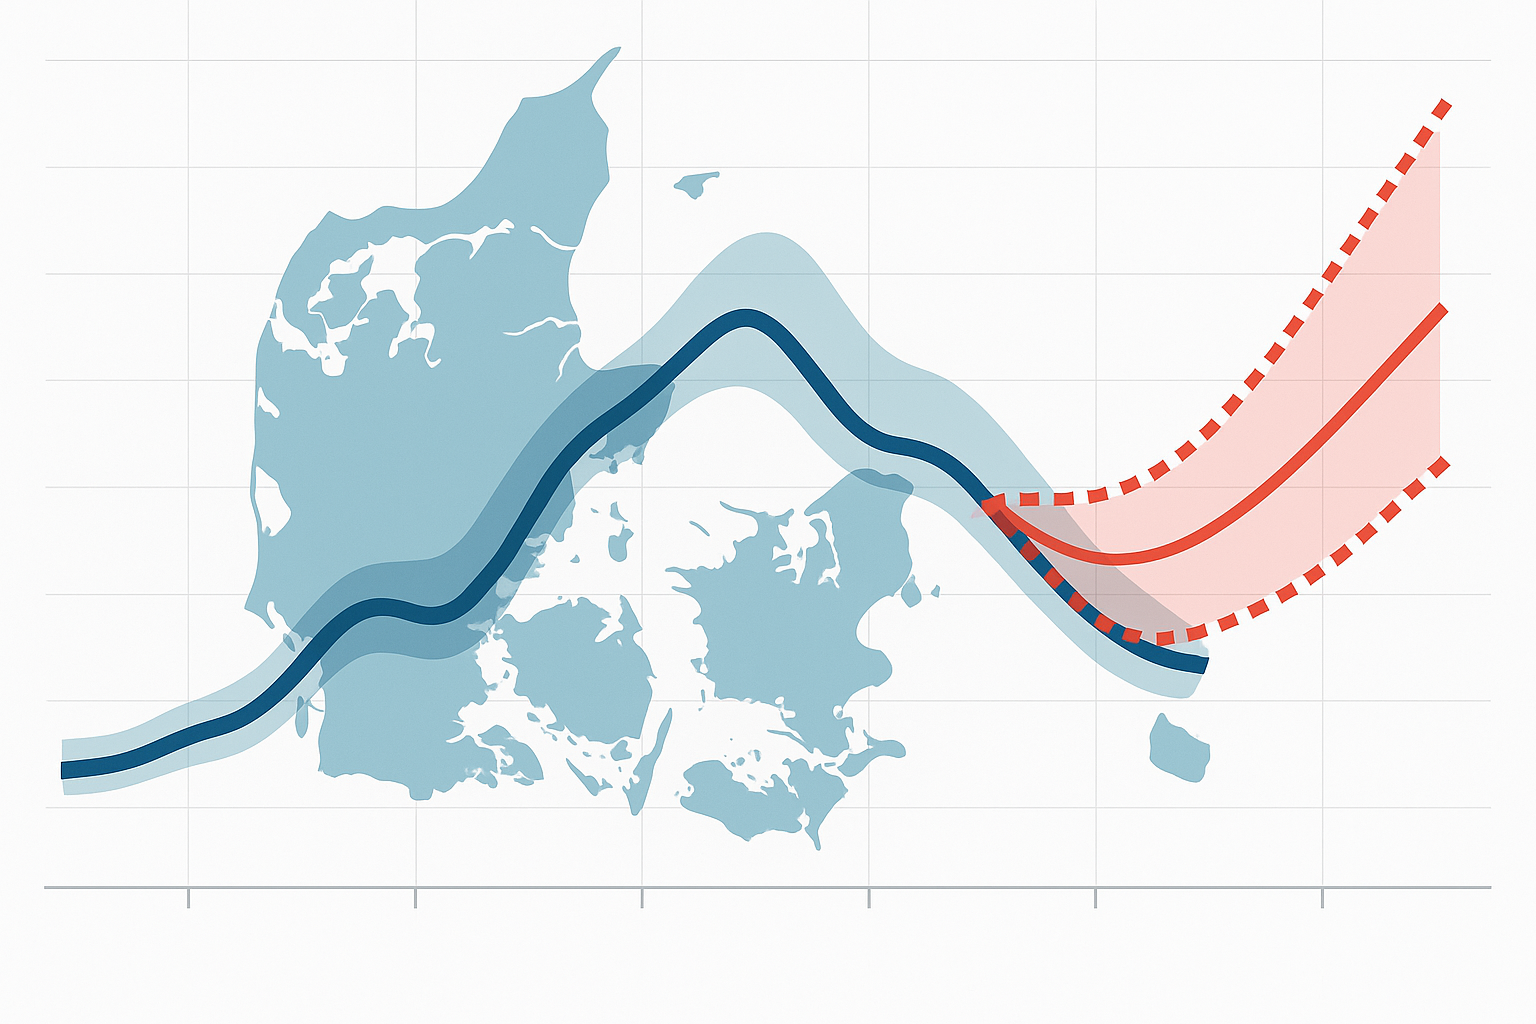
\includegraphics[width=0.9\textwidth]{fotos/forside.png} \\[2em]
\end{center}
\begin{center}
\fcolorbox{gray}{white}{
\parbox{0.8\textwidth}{
\centering
\textbf{Antal tegn (inkl. mellemrum): 32.000}
}}
\end{center}
\begin{center}
\textbf{Vejledere:} \\
Bjarne Taulo Sørensen \\
\end{center}

\newpage

\tableofcontents

\pagenumbering{arabic}
\setcounter{page}{1}
\newpage

\section{Introduktion}\label{introduktion}

Arbejdsløshedstal er en central indikator for et lands økonomiske
tilstand og udvikling. De påvirker både den enkelte borger og den
nationale økonomi og indgår som en væsentlig faktor i politiske og
økonomiske beslutningsprocesser. I takt med øget datatilgængelighed og
forbedrede statistiske værktøjer er det blevet muligt at analysere og
forudsige sådanne udviklingstræk med større præcision.

Denne opgave undersøger arbejdsløshedens udvikling i Danmark fra 2007
til 2019, fordelt på køn og region. Datagrundlaget består af ti
tidsserier, der dækker hver kombination af fem regioner og to køn. Det
giver mulighed for at analysere både regionale forskelle og
kønsspecifikke mønstre i arbejdsløsheden.

Analysen baseres på tre klassiske modeltyper: ARIMA, ETS og en enkel
benchmarkmodel (Seasonal Naive). Modellerne anvendes til at undersøge
historiske tendenser og fremskrive udviklingen. Undervejs vurderes
modellernes egnethed med fokus på præcision og residualstruktur, og der
anvendes teknikker som STL-dekomposition og transformation af data.
Målet er ikke blot at forudsige udviklingen i 2020, men også at vurdere,
hvor godt klassiske modeller formår at håndtere forskellene mellem
regioner og køn.

\section{Problemformulering}\label{problemformulering}

Hvordan kan klassiske tidsseriemodeller anvendes til at analysere og
forudsige udviklingen i arbejdsløsheden i Danmark, fordelt på region og
køn?

For at besvare dette spørgsmål undersøges følgende delspørgsmål:

\begin{enumerate}
\def\labelenumi{\arabic{enumi}.}
\item
  Hvordan varierer arbejdsløshedens udvikling og sæsonmønstre på tværs
  af regioner og køn, og hvordan kan disse identificeres gennem
  eksplorativ dataanalyse og dekomposition?
\item
  Hvordan performer modellerne ARIMA, ETS og Seasonal Naive i forhold
  til hinanden, når det gælder præcision, residualstruktur og
  prognoseegenskaber?
\item
  Hvilke modeller er bedst egnede til at fremskrive
  arbejdsløshedstallene for 2020, og hvordan varierer usikkerheden på
  tværs af serier?
\end{enumerate}

\subsection{Afgrænsning}\label{afgruxe6nsning}

Analysen baserer sig udelukkende på de udleverede arbejdsløshedstal for
perioden januar 2007 til december 2019 og anvender ingen eksterne
forklaringsvariable såsom COVID-19, økonomiske indikatorer eller
politiske reformer. Formålet er at isolere de metodiske egenskaber ved
modellerne og vurdere deres evne til at håndtere mønstre i selve
tidsserierne. Fokus er således på statistisk modellering og forecast --
ikke på årsagsforklaringer eller samfundsøkonomiske vurderinger.

\subsubsection{Anvendelse af
AI-værktøj}\label{anvendelse-af-ai-vuxe6rktuxf8j}

ChatGPT (GPT-4o) er anvendt som støtteværktøj i forbindelse med
idéudvikling, sproglig formulering og udformning af kodestumper.
Værktøjet er kun brugt til tekniske og sproglige formål. Det
understreges derfor at al analyse, fortolkning og konklusion er
udarbejdet selvstændigt af gruppens medlemmer.

\subsection{Definitioner/forkortelser}\label{definitionerforkortelser}

Nedenfor er en oversigt over centrale begreber og forkortelser, som
anvendes i opgaven:

\begin{itemize}
\tightlist
\item
  \textbf{ARIMA}: AutoRegressive Integrated Moving Average
\item
  \textbf{ETS}: Exponential Smoothing State Space Model
\item
  \textbf{SNAÏVE}: Seasonal Naive
\item
  \textbf{RMSE}: Root Mean Squared Error
\item
  \textbf{MAPE}: Mean Absolute Percentage Error
\item
  \textbf{STL}: Seasonal-Trend decomposition using Loess
\item
  \textbf{CV}: Cross-validation
\end{itemize}

\subsection{Struktur}\label{struktur}

Opgavens struktur følger en klassisk tilgang til tidsserieanalyse og er
inddelt i fem faser. Først gennemføres en eksplorativ dataanalyse med
fokus på mønstre og variationer i arbejdsløsheden fordelt på region og
køn. Dernæst estimeres tre modeller (ARIMA, ETS og Seasonal Naive) for
hver tidsserie. I tredje fase valideres modellerne gennem
krydsvalidering og residualanalyse. Herefter foretages fremskrivninger
for 2020, og til sidst sammenlignes og konkluderes der på tværs af
modeller og dataserier.

\section{Data og forberedelse}\label{data-og-forberedelse}

Analysen bygger på månedlige arbejdsløshedstal fra Danmark i perioden
januar 2007 til december 2019. Data er opdelt efter køn og region,
hvilket giver ti separate tidsserier. Datasættet er udleveret i et
forbehandlet tsibble-format med tydeligt definerede indeks- og
nøglevariabler. Nedenfor vises indlæsningen af datasættet:

\begin{verbatim}
# A tsibble: 6 x 4 [1M]
# Key:       kon, region [1]
  kon     region             yearmonth svalue
  <fct>   <fct>                  <mth>  <dbl>
1 Kvinder Region Hovedstaden  2007 Jan   2.26
2 Kvinder Region Hovedstaden  2007 Feb   2.19
3 Kvinder Region Hovedstaden  2007 Mar   2.09
4 Kvinder Region Hovedstaden  2007 Apr   1.97
5 Kvinder Region Hovedstaden  2007 May   1.99
6 Kvinder Region Hovedstaden  2007 Jun   1.93
\end{verbatim}

\section{Eksplorativ dataanalyse
(EDA)}\label{eksplorativ-dataanalyse-eda}

Formålet med dette afsnit er at skabe et overblik over datasættets
struktur forud for modelleringen. Ved hjælp af visualiseringer,
deskriptive statistikker og STL-dekomposition undersøges
arbejdsløshedens udvikling på tværs af regioner og køn i perioden 2007
til 2019. Analysen afdækker overordnede tendenser, sæsonmønstre og
forskelle i niveau og variation. Resultaterne danner det metodiske
fundament for det videre modelarbejde.

\subsection{Visualisering af udvikling og
mønstre}\label{visualisering-af-udvikling-og-muxf8nstre}

I dette afsnit undersøges, hvordan arbejdsløsheden har udviklet sig over
tid med fokus på tendenser, sæsonvariationer og forskelle mellem
regioner og køn. Formålet er at identificere mønstre, som kan guide valg
af modeller i den videre analyse.

\subsubsection{Udvikling over tid}\label{udvikling-over-tid}

I de følgende figurer undersøges udviklingen i arbejdsløsheden over tid.
Til at begynde med anvendes den oprindelige skala for at give et
lettilgængeligt overblik (Figur 1). Fra Figur 2 og frem benyttes en
log-transformation for at stabilisere variationen i serierne, især
blandt mænd, og for at sikre sammenlignelighed i videre modellering og
forecast.

\pandocbounded{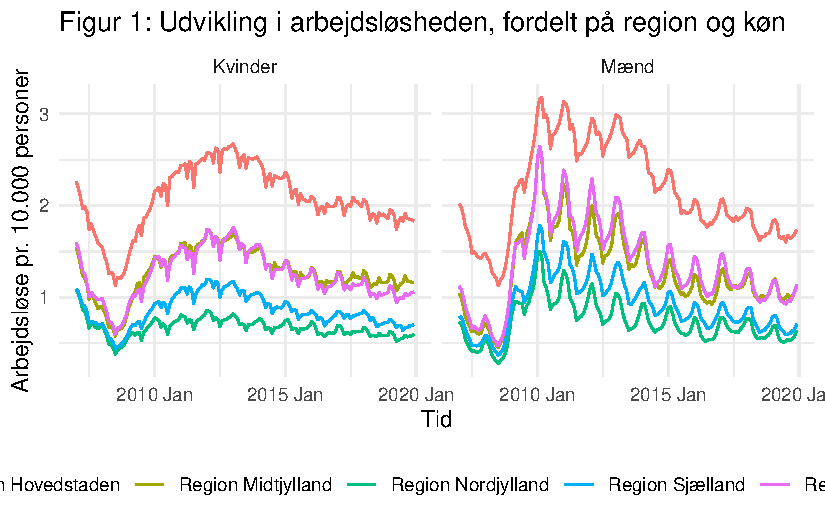
\includegraphics[keepaspectratio]{130625_Forecasting_files/figure-pdf/figur 1-1.pdf}}

Figur 1 viser udviklingen i arbejdsløsheden fra 2007 til 2019 for begge
køn i alle fem regioner. Der tegner sig et tydeligt sæsonmønster med
højere ledighed i vintermånederne og lavere i sommerperioden. Region
Hovedstaden har generelt højere ledighedsniveau, mens Nordjylland og
Sjælland ligger lavere. Efter finanskrisen ses en gradvis nedgang i
ledigheden i næsten alle grupper.

\pandocbounded{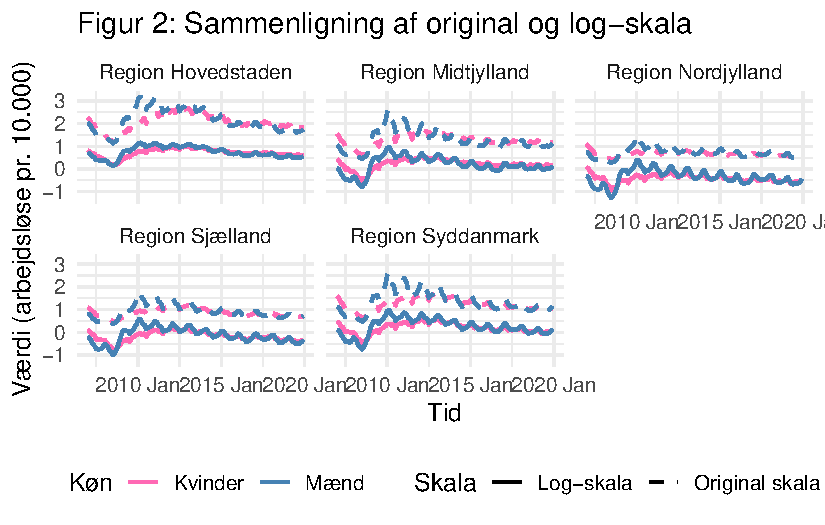
\includegraphics[keepaspectratio]{130625_Forecasting_files/figure-pdf/figur 2-1.pdf}}

Figur 2 viser, hvordan log-transformeringen dæmper udsvingene, særligt i
serier med højt niveau og stor variation, som det ses blandt mænd. Denne
transformation gør det lettere at sammenligne udviklingen på tværs af
regioner og køn og sikrer en mere stabil varians i det videre
analysearbejde. Derfor anvendes den log-transformerede version
fremadrettet i analysen.

\subsubsection{Sæsonmønstre}\label{suxe6sonmuxf8nstre}

Med log-transformerede data som fundament undersøges nu sæsonmønstrene i
arbejdsløsheden nærmere. Gennem sæsonplots og subserieplots vurderes,
hvordan arbejdsløsheden typisk varierer over året -- og hvordan dette
adskiller sig mellem mænd og kvinder samt på tværs af regioner.

\pandocbounded{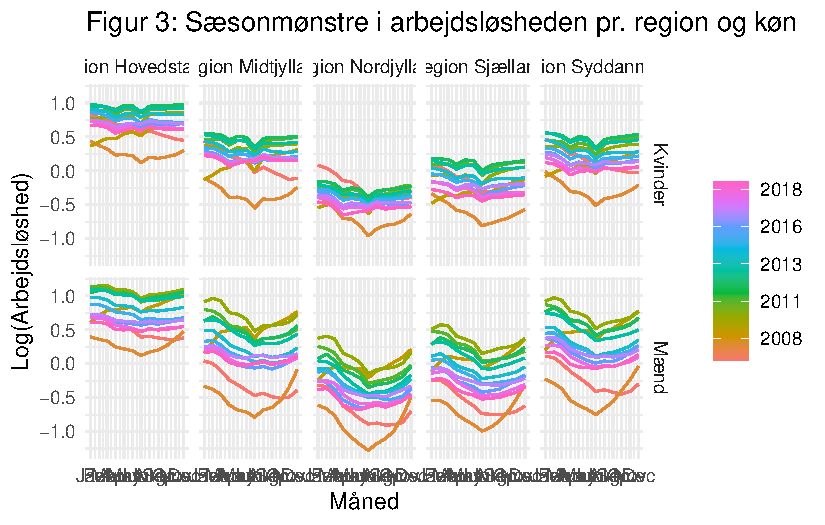
\includegraphics[keepaspectratio]{130625_Forecasting_files/figure-pdf/figur 3-1.pdf}}

Figur 3 viser sæsonmønstre i arbejdsløsheden fordelt på region og køn
(logtransformeret). Hver farve repræsenterer et år. Der ses et klart
mønster med høj ledighed i årets begyndelse og lav i sommermånederne.
Mænd har generelt større udsving end kvinder. Niveauet er højest i
Hovedstaden og lavest i Nordjylland og Sjælland. Negative logværdier
optræder, når arbejdsløsheden ligger under én pr. 10.000.

\pandocbounded{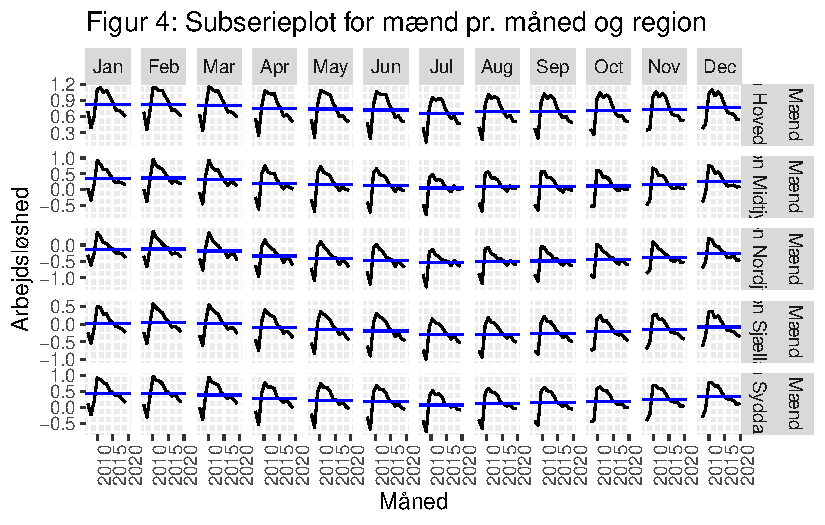
\includegraphics[keepaspectratio]{130625_Forecasting_files/figure-pdf/figur 4-1.pdf}}

Figur 4 viser subserieplot for mænd, hvor hver celle viser udviklingen i
én måned over årene. Sorte linjer angiver observationer, blå linjer
gennemsnit. Der ses høj ledighed i årets første måneder og fald hen over
sommeren. Mænd har større sæsonudsving og højere variation mellem år,
især i vinterhalvåret.

\pandocbounded{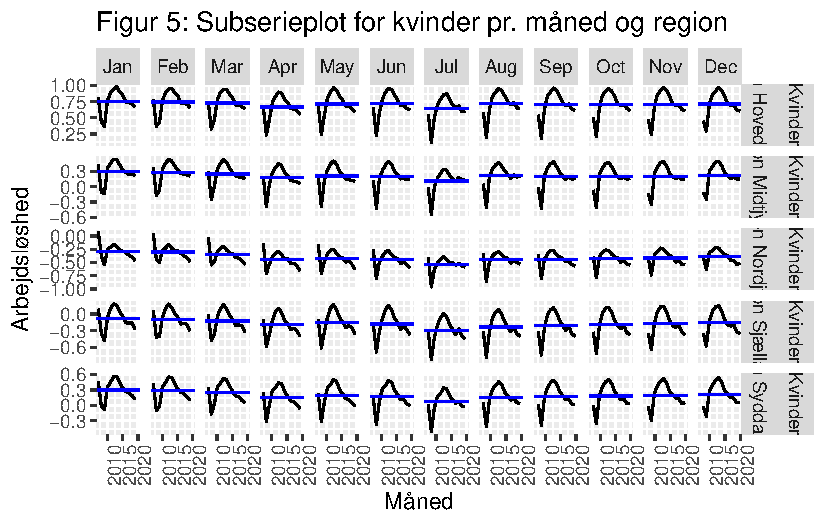
\includegraphics[keepaspectratio]{130625_Forecasting_files/figure-pdf/figur 5-1.pdf}}

Tilsvarende viser Figur 5 sæsonmønstre for kvinder. Mønstret er det
samme som for mænd, men udsvingene er mindre. Forskellene mellem år er
mindre tydelige. Udviklingen er mere stabil og jævnt fordelt, hvilket
tyder på lavere variation i kvinders arbejdsløshed.

For at underbygge disse visuelle indsigter med konkrete tal, præsenteres
i næste afsnit deskriptive statistikker. De giver en numerisk
opsummering af centrale mål som gennemsnit, variation og ekstreme
værdier og bidrager til at identificere særligt stabile eller volatile
grupper, der kan kræve særlig opmærksomhed i den videre analyse.

\subsection{Deskriptive statistikker}\label{deskriptive-statistikker}

De foregående visualiseringer viste klare forskelle i arbejdsløshedens
niveau, variation og sæsonmønstre på tværs af regioner og køn (Figur
1--5). For at supplere disse observationer med en kvantitativ
opsummering præsenteres i Tabel 1 centrale deskriptive mål: gennemsnit,
standardafvigelse, minimum og maksimum. Tabellen giver et hurtigt
overblik over niveau og variation og fremhæver for eksempel Nordjylland
som en stabil region, særligt blandt kvinder, mens andre kombinationer
viser højere udsving.

\begin{longtable}[t]{llrrrr}
\caption{Deskriptiv statistik per region og køn}\\
\toprule
\cellcolor[HTML]{f0f0f0}{\textbf{region}} & \cellcolor[HTML]{f0f0f0}{\textbf{kon}} & \cellcolor[HTML]{f0f0f0}{\textbf{Gennemsnit}} & \cellcolor[HTML]{f0f0f0}{\textbf{Standardafvigelse}} & \cellcolor[HTML]{f0f0f0}{\textbf{Minimum}} & \cellcolor[HTML]{f0f0f0}{\textbf{Maksimum}}\\
\midrule
Region Hovedstaden & Kvinder & 2.07 & 0.36 & 1.13 & 2.67\\
Region Hovedstaden & Mænd & 2.17 & 0.52 & 1.13 & 3.18\\
Region Midtjylland & Kvinder & 1.27 & 0.25 & 0.58 & 1.72\\
Region Midtjylland & Mænd & 1.29 & 0.44 & 0.45 & 2.62\\
Region Nordjylland & Kvinder & 0.67 & 0.10 & 0.38 & 1.09\\
\addlinespace
Region Nordjylland & Mænd & 0.74 & 0.23 & 0.28 & 1.50\\
Region Sjælland & Kvinder & 0.86 & 0.17 & 0.45 & 1.20\\
Region Sjælland & Mænd & 0.92 & 0.30 & 0.37 & 1.78\\
Region Syddanmark & Kvinder & 1.24 & 0.26 & 0.60 & 1.76\\
Region Syddanmark & Mænd & 1.37 & 0.47 & 0.47 & 2.65\\
\bottomrule
\end{longtable}

\subsubsection{Features}\label{features}

Selvom deskriptive statistikker giver et første indtryk af variation og
niveau, indfanger de ikke strukturelle træk som trend, sæsonmønstre og
stationaritet. For at kvantificere disse egenskaber beregnes en række
såkaldte features ved hjælp af ved hjælp af funktionen features() fra
feasts-pakken (Hyndman \& Athanasopoulos, 2021, kap. 4).

Tabel 2 præsenterer udvalgte mål, der beskriver centrale træk ved
serierne og uddyber de visuelle indsigter fra Figur 1--5. Den
bagvedliggende kode, herunder brugen af features()-funktionen og
indlæsning af dataobjektet feature\_table.rds, er dokumenteret i Bilag
1.

\begin{longtable}[t]{llrrrrrr}
\caption{Deskriptiv statistik per region og køn}\\
\toprule
\cellcolor[HTML]{f0f0f0}{\textbf{kon}} & \cellcolor[HTML]{f0f0f0}{\textbf{region}} & \cellcolor[HTML]{f0f0f0}{\textbf{acf1}} & \cellcolor[HTML]{f0f0f0}{\textbf{seasonal\_strength\_year}} & \cellcolor[HTML]{f0f0f0}{\textbf{var\_tiled\_mean}} & \cellcolor[HTML]{f0f0f0}{\textbf{shift\_level\_max}} & \cellcolor[HTML]{f0f0f0}{\textbf{ndiffs}} & \cellcolor[HTML]{f0f0f0}{\textbf{trend\_strength}}\\
\midrule
Kvinder & Region Hovedstaden & 0.97 & 0.65 & 0.97 & 0.38 & 1 & 0.99\\
Kvinder & Region Midtjylland & 0.96 & 0.72 & 0.92 & 0.54 & 1 & 0.98\\
Kvinder & Region Nordjylland & 0.89 & 0.87 & 0.73 & 0.47 & 0 & 0.97\\
Kvinder & Region Sjælland & 0.96 & 0.81 & 0.92 & 0.43 & 1 & 0.99\\
Kvinder & Region Syddanmark & 0.96 & 0.83 & 0.91 & 0.45 & 1 & 0.99\\
\addlinespace
Mænd & Region Hovedstaden & 0.98 & 0.81 & 0.98 & 0.58 & 1 & 0.99\\
Mænd & Region Midtjylland & 0.98 & 0.84 & 0.93 & 1.05 & 0 & 0.98\\
Mænd & Region Nordjylland & 0.96 & 0.91 & 0.80 & 0.89 & 0 & 0.97\\
Mænd & Region Sjælland & 0.97 & 0.92 & 0.90 & 0.80 & 1 & 0.99\\
Mænd & Region Syddanmark & 0.98 & 0.88 & 0.91 & 0.96 & 1 & 0.98\\
\bottomrule
\end{longtable}

De kvantitative mål i Tabel 2 supplerer og styrker tolkningerne fra
Figur 1 til 5. I det følgende fremhæves de mest centrale mønstre med
fokus på fem analytiske temaer: autokorrelation, sæsonmønstre, variation
og skift, stationaritet og trend.

\textbf{Autokorrelation}

Variablen acf1 måler korttidsafhængighed, det vil sige, hvor stærkt
observationer i serien er knyttet til deres nære fortid. Værdierne
ligger generelt højt (typisk mellem 0,96 og 0,98), hvilket indikerer en
glidende udvikling uden pludselige udsving. Dette stemmer overens med de
jævne bevægelser og stabile tendenser, som blev observeret i Figur 1 og
Figur 2.

\textbf{Sæsonmønstre}

Styrken af årlige sæsonmønstre, målt med seasonal\_strength\_year,
varierer på tværs af grupper. Mænd udviser generelt mere udtalte
sæsonudsving end kvinder. For eksempel har mænd i Nordjylland og
Sjælland værdier på henholdsvis 0,91 og 0,92. Det svarer til de tydelige
sæsonrytmer vist i Figur 3, Figur 4 og Figur 5. I modsætning hertil har
kvinder i Region Hovedstaden en lavere værdi på 0,65, hvilket indikerer
en mere stabil sæsonprofil.

\textbf{Variation og skift}

Målet var\_tiled\_mean afspejler graden af variation inden for
afgrænsede perioder. Kvinder i Nordjylland har den laveste værdi (0,73),
hvilket viser en forholdsvis stabil udvikling over tid. Dette
understøttes af de glatte kurver i Figur 5. Variablen shift\_level\_max
måler derimod pludselige niveauskift. Mænd i Midtjylland udviser den
højeste værdi (1,05), hvilket sandsynligvis relaterer sig til reaktioner
på finanskrisen og kan ses i de kraftige fald i arbejdsløsheden i Figur
1 og Figur 2.

\textbf{Stationaritet}

Antallet af nødvendige differensieringer (ndiffs) angiver, hvorvidt en
serie er stationær. De fleste serier kræver én differens, men enkelte,
herunder kvinder i Nordjylland og mænd i både Midtjylland og
Nordjylland, har værdi 0. Dette indikerer, at de allerede er stationære
uden transformation, hvilket også kommer til udtryk i deres stabile
forløb i Figur 3 og Figur 5.

\textbf{Trend}

Variablen trend\_strength måler graden af trendstruktur i serien.
Værdierne ligger generelt meget højt (typisk 0,97 til 0,99), hvilket
bekræfter tydelige underliggende tendenser i arbejdsløsheden. Det gælder
især Region Hovedstaden, hvor niveauet er højt, og udviklingen over tid
er markant, som det fremgår af Figur 1 og Figur 2.

Samlet set bidrager funktionerne i Tabel 2 til at kvantificere og
validere de mønstre, der tidligere blev identificeret visuelt.
Autokorrelation, sæsonvariation og trendstruktur fremstår som
gennemgående karakteristika i alle serier, men med klare forskelle
mellem køn og regioner. Resultaterne danner et vigtigt grundlag for valg
af modeller og videre analyse.

\subsection{STL-dekomposition}\label{stl-dekomposition}

STL-dekomposition anvendes for at undersøge de strukturelle komponenter
i arbejdsløshedsserierne. Metoden opdeler tidsserierne i tre dele:
trend, sæson og remainder, hvilket giver indblik i, hvor stor en del af
variationen der skyldes henholdsvis langsigtet udvikling,
tilbagevendende mønstre eller kortsigtede udsving (Hyndman og
Athanasopoulos, 2021). Dekompositionen er udført separat for mænd og
kvinder i hver region, og resultaterne vises i figur 6 og 7.

\pandocbounded{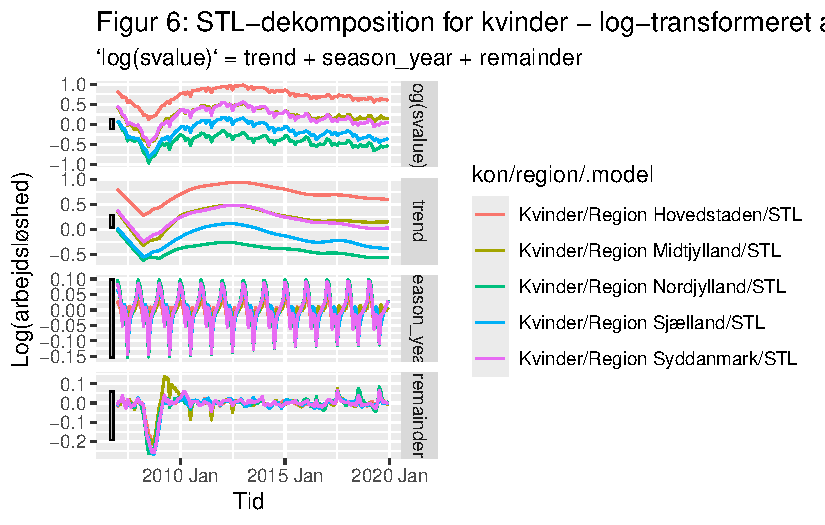
\includegraphics[keepaspectratio]{130625_Forecasting_files/figure-pdf/figur 6-1.pdf}}

Figur 6 viser STL-dekompositionen for kvinder i de fem danske regioner.
Der ses tydelige sæsonmønstre med tilbagevendende lavpunkter i
sommermånederne og højere ledighed i vinterhalvåret. Trends varierer
mellem regionerne: Region Hovedstaden udviser generelt højere ledighed,
mens Nordjylland og Sjælland ligger lavere. Residualerne ligger stabilt
omkring nul, hvilket indikerer, at modellen formår at fange de
dominerende strukturer i data.

\pandocbounded{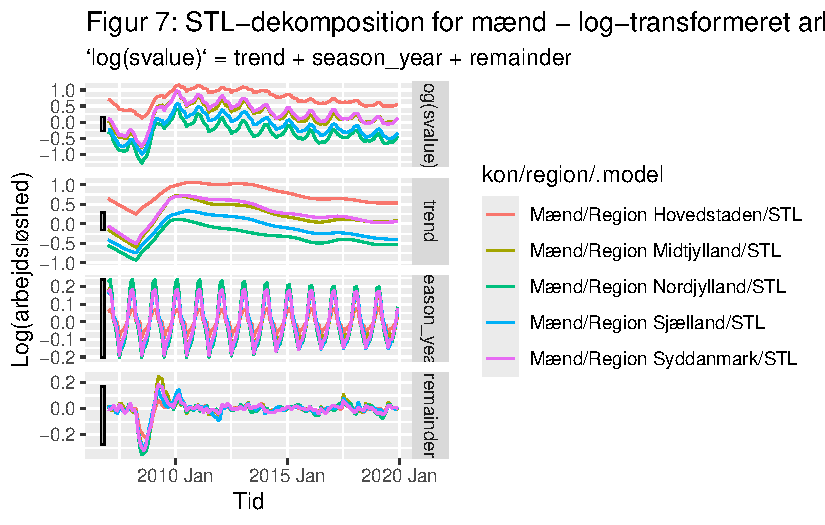
\includegraphics[keepaspectratio]{130625_Forecasting_files/figure-pdf/unnamed-chunk-2-1.pdf}}

Figur 7 viser tilsvarende dekomposition for mænd. Her ses en tilsvarende
stærk sæsonkomponent, men med mere markante udsving og højere
ledighedsniveauer -- især efter finanskrisen. Trends følger samme
overordnede forløb som for kvinder, men afvigelserne er større. Dette
bekræfter tidligere observationer om højere volatilitet i mænds
ledighed. Residualkomponenten er mere varierende, hvilket kan indikere,
at nogle udsving ikke fanges fuldt ud af modellen.

Disse observationer fra STL-dekompositionen bekræfter, at både trend og
sæsonmønstre varierer betydeligt på tværs af serierne. Det understreger
behovet for modeller, der kan tilpasses hver series struktur, hvilket
vil blive præsenteret i det følgende afsnit.

\section{Modelvalg}\label{modelvalg}

I dette afsnit præsenteres tre klassiske modeltyper: ARIMA, ETS og
benchmarkmodellen SNaive. Hver model estimeres for de ti tidsserier, der
er defineret som kombinationer af region og køn. Modellerne adskiller
sig i deres antagelser og egenskaber og er hver især velegnede til at
fange strukturelle mønstre som trend, sæson og autokorrelation.
Estimeringen foretages automatisk med fable-pakken, som vælger den bedst
egnede specifikation for hver serie. Den endelige vurdering af
modellernes præcision og egnethed gennemføres i næste afsnit.

\subsection{Valgte modeltyper}\label{valgte-modeltyper}

\textbf{ARIMA (AutoRegressive Integrated Moving Average)}\\
ARIMA-modeller anvendes til at modellere tidsserier med autokorrelation
og ikke-stationaritet. De kombinerer autoregressive (AR) led, differens
(I) for at opnå stationaritet, og glidende gennemsnit (MA) led til at
modellere fejl. Ved at inkludere sæsonkomponenter (SARIMA) kan modellen
håndtere årligt gentagende mønstre. ARIMA er særligt velegnet til serier
med langsigtede trends og strukturelle skift, hvor tidligere værdier har
stor indflydelse på den nuværende tilstand (Hyndman \& Athanasopoulos,
2021, kap. 9).

\textbf{ETS (Exponential Smoothing State Space Model)}\\
ETS-modeller benytter eksponentiel glatning til at vægte nyere
observationer højere og beskriver tidsserier ud fra tre elementer: fejl,
trend og sæson. Hver komponent kan være additiv eller multiplicativ
afhængigt af dataens karakter. ETS egner sig godt til serier med
tydelige strukturer og sæsonrytmer, især når der ikke er behov for at
modellere autokorrelation direkte (Hyndman \& Athanasopoulos, 2021, kap.
8).

\textbf{SNAÏVE (Seasonal Naive)}\\
SNaive er en simpel sammenligningsmodel, der baserer hvert forecast på
den tilsvarende værdi fra samme sæson i den foregående periode. Modellen
fanger sæsonmønstre, men tager ikke højde for trend eller afhængighed i
data. Den anvendes til at vurdere, om mere komplekse modeller giver en
mærkbart bedre forecast-præcision (Hyndman \& Athanasopoulos, 2021, kap.
3 og 8).

\section{Modelvalidering}\label{modelvalidering}

Dette afsnit har til formål at sikre, at modellerne giver pålidelige
fremskrivninger og ikke blot tilpasser sig historiske data. Der anvendes
time series cross-validation, og modellerne evalueres ved hjælp af
metrikker som RMSE og MAPE. På baggrund af dette identificeres den bedst
egnede model for hver tidsserie. Derudover foretages residualanalyse for
at undersøge, om der er tegn på hvid støj, hvilket er en forudsætning
for valide modeller.

\subsection{Opdeling af data i træning og
test}\label{opdeling-af-data-i-truxe6ning-og-test}

Datasættet opdeles i to perioder for at kunne evaluere modellernes
præcision på nye observationer. Træningssættet dækker perioden januar
2007 til december 2018, mens testsættet består af data fra januar til
december 2019. Denne opdeling gør det muligt at sammenligne modellerne
på ens vilkår og vurdere deres evne til at generalisere.

\begin{Shaded}
\begin{Highlighting}[]
\NormalTok{train\_data }\OtherTok{\textless{}{-}}\NormalTok{ data }\SpecialCharTok{|\textgreater{}} \FunctionTok{filter\_index}\NormalTok{(. }\SpecialCharTok{\textasciitilde{}} \StringTok{"2018 Dec"}\NormalTok{)}
\NormalTok{test\_data  }\OtherTok{\textless{}{-}}\NormalTok{ data }\SpecialCharTok{|\textgreater{}} \FunctionTok{filter\_index}\NormalTok{(}\StringTok{"2019 Jan"} \SpecialCharTok{\textasciitilde{}} \StringTok{"2019 Dec"}\NormalTok{)}
\end{Highlighting}
\end{Shaded}

\subsection{Time series
cross-validation}\label{time-series-cross-validation}

For at vurdere modellernes forecast-præcision anvendes time series
cross-validation på træningsdata. Et rullende vindue på 60 måneder
anvendes til at generere flere trænings- og test-split, forskudt én
måned ad gangen. Der anvendes stretch\_tsibble() til at generere flere
trænings- og test-split, som forskydes én måned ad gangen. Tre modeller
evalueres: ARIMA, ETS og SNaive.

Alle modeller estimeres på logtransformerede data. Forecastfejlene
beregnes med accuracy(), og beregningerne køres parallelt for hurtigere
eksekvering. Resultaterne gemmes med write\_rds() for reproducérbarhed.

\begin{Shaded}
\begin{Highlighting}[]
\CommentTok{\# plan(multisession)}

\CommentTok{\# cv\_data \textless{}{-} train\_data |\textgreater{}}
\CommentTok{\#   stretch\_tsibble(.init = 60, .step = 1)}

\CommentTok{\# cv\_models \textless{}{-} cv\_data |\textgreater{}}
\CommentTok{\#   model(}
\CommentTok{\#     ARIMA  = ARIMA(log(svalue)),}
\CommentTok{\#     ETS    = ETS(log(svalue)),}
\CommentTok{\#     SNaive = SNAIVE(log(svalue))}
\CommentTok{\#   )}

\CommentTok{\# write\_rds(cv\_models, "cv\_models.rds")}

\NormalTok{cv\_models }\OtherTok{\textless{}{-}} \FunctionTok{read\_rds}\NormalTok{(}\StringTok{"data/cv\_models.rds"}\NormalTok{)}

\NormalTok{cv\_accuracy }\OtherTok{\textless{}{-}}\NormalTok{ cv\_models }\SpecialCharTok{|\textgreater{}}
  \FunctionTok{accuracy}\NormalTok{()}

\CommentTok{\# plan(sequential)}
\end{Highlighting}
\end{Shaded}

\subsubsection{Valg af den bedst præsterende
model}\label{valg-af-den-bedst-pruxe6sterende-model}

Her identificeres den bedste model for hver kombination af køn og region
baseret på laveste RMSE. Ved at gruppere på kon og region og vælge
modellen med mindst fejl (slice\_min()), får vi én vinder pr. serie uden
ligestilling mellem modeller (with\_ties = FALSE). Dette gør det muligt
senere at bruge den bedste model til forecast for hver delserie.

\begin{Shaded}
\begin{Highlighting}[]
\NormalTok{vinder\_cv }\OtherTok{\textless{}{-}}\NormalTok{ cv\_accuracy }\SpecialCharTok{|\textgreater{}}
  \FunctionTok{group\_by}\NormalTok{(kon, region) }\SpecialCharTok{|\textgreater{}}
  \FunctionTok{slice\_min}\NormalTok{(RMSE, }\AttributeTok{n =} \DecValTok{1}\NormalTok{, }\AttributeTok{with\_ties =} \ConstantTok{FALSE}\NormalTok{) }\SpecialCharTok{|\textgreater{}}
  \FunctionTok{ungroup}\NormalTok{()}

\NormalTok{vinder\_cv }\SpecialCharTok{|\textgreater{}} \FunctionTok{select}\NormalTok{(kon, region, .model)}
\end{Highlighting}
\end{Shaded}

\begin{verbatim}
# A tibble: 10 x 3
   kon     region             .model
   <fct>   <fct>              <chr> 
 1 Kvinder Region Hovedstaden ETS   
 2 Kvinder Region Midtjylland ARIMA 
 3 Kvinder Region Nordjylland ARIMA 
 4 Kvinder Region Sjælland    ARIMA 
 5 Kvinder Region Syddanmark  ARIMA 
 6 Mænd    Region Hovedstaden ARIMA 
 7 Mænd    Region Midtjylland ARIMA 
 8 Mænd    Region Nordjylland ARIMA 
 9 Mænd    Region Sjælland    ARIMA 
10 Mænd    Region Syddanmark  ARIMA 
\end{verbatim}

Resultaterne viser, at ARIMA-modellen klarer sig bedst i 9 ud af 10
tidsserier. Den eneste undtagelse er kvinder i Region Hovedstaden, hvor
en ETS-model giver lavest RMSE. Dette tyder på, at ARIMA generelt formår
at tilpasse sig strukturen i dataserierne bedre, hvilket ofte skyldes
modellens fleksibilitet i forhold til både trend og sæson. Den ene
ETS-vinder indikerer dog, at i nogle tilfælde kan eksponentiel glatning
være mere passende -- muligvis pga. mere stabil sæson uden kompleks
autokorrelation.

\subsection{Forecast for 2019 med
vinder-modeller}\label{forecast-for-2019-med-vinder-modeller}

Når den bedst præsterende model er udpeget for hver tidsserie via
cross-validation, trænes alle tre modeller (ARIMA, ETS og SNaive) på
hele træningsperioden fra januar 2007 til december 2018. Herefter laves
et 12-måneders forecast for 2019.

Forecastet baseres kun på den tidligere udpegede vinder for hver serie,
hvilket sikres ved at filtrere resultatet med inner\_join() mod
vinder\_cv.

\begin{Shaded}
\begin{Highlighting}[]
\NormalTok{model\_train }\OtherTok{\textless{}{-}}\NormalTok{ train\_data }\SpecialCharTok{|\textgreater{}}
  \FunctionTok{model}\NormalTok{(}
    \AttributeTok{ARIMA  =} \FunctionTok{ARIMA}\NormalTok{(}\FunctionTok{log}\NormalTok{(svalue)),}
    \AttributeTok{ETS    =} \FunctionTok{ETS}\NormalTok{(}\FunctionTok{log}\NormalTok{(svalue)),}
    \AttributeTok{SNaive =} \FunctionTok{SNAIVE}\NormalTok{(}\FunctionTok{log}\NormalTok{(svalue))}
\NormalTok{  )}

\NormalTok{train\_accuracy }\OtherTok{\textless{}{-}}\NormalTok{ model\_train }\SpecialCharTok{|\textgreater{}} 
  \FunctionTok{accuracy}\NormalTok{() }\SpecialCharTok{|\textgreater{}} 
  \FunctionTok{select}\NormalTok{(kon, region, .model, }\AttributeTok{RMSE\_tr =}\NormalTok{ RMSE, }\AttributeTok{MAPE\_tr =}\NormalTok{ MAPE)}

\NormalTok{forecast\_2019 }\OtherTok{\textless{}{-}}\NormalTok{ model\_train }\SpecialCharTok{|\textgreater{}}
  \FunctionTok{forecast}\NormalTok{(}\AttributeTok{h =} \StringTok{"12 months"}\NormalTok{) }\SpecialCharTok{|\textgreater{}}
  \FunctionTok{inner\_join}\NormalTok{(vinder\_cv,                      }
             \AttributeTok{by =} \FunctionTok{c}\NormalTok{(}\StringTok{"kon"}\NormalTok{, }\StringTok{"region"}\NormalTok{, }\StringTok{".model"}\NormalTok{))}
\end{Highlighting}
\end{Shaded}

Forecastet for 2019 baseres dermed på den model, som tidligere blev
vurderet som bedst egnet til den enkelte serie. Dette danner grundlag
for at sammenligne modellens præcision på træningsdata og dens evne til
at generalisere til nye observationer i testsættet.

\subsection{Sammenligning af trænings- og
testfejl}\label{sammenligning-af-truxe6nings--og-testfejl}

For at vurdere modellernes evne til at generalisere sammenlignes
forecastfejl på trænings- og testdata. Dette gøres ved at kombinere de
to i én samlet tabel (train\_vs\_test), hvor RMSE og MAPE for hver serie
fremgår.

\begin{verbatim}
# A tibble: 10 x 7
   kon     region             .model RMSE_tr   RMSE MAPE_tr  MAPE
   <fct>   <fct>              <chr>    <dbl>  <dbl>   <dbl> <dbl>
 1 Kvinder Region Hovedstaden ETS     0.0434 0.0398    1.68  1.82
 2 Kvinder Region Midtjylland ARIMA   0.0290 0.0436    1.70  3.43
 3 Kvinder Region Nordjylland ARIMA   0.0133 0.0122    1.46  1.72
 4 Kvinder Region Sjælland    ARIMA   0.0156 0.0280    1.28  2.88
 5 Kvinder Region Syddanmark  ARIMA   0.0238 0.0236    1.41  1.85
 6 Mænd    Region Hovedstaden ARIMA   0.0383 0.0784    1.26  4.13
 7 Mænd    Region Midtjylland ARIMA   0.0503 0.0193    2.41  1.52
 8 Mænd    Region Nordjylland ARIMA   0.0296 0.0140    2.49  2.00
 9 Mænd    Region Sjælland    ARIMA   0.0289 0.0153    1.94  1.85
10 Mænd    Region Syddanmark  ARIMA   0.0464 0.0846    2.12  6.86
\end{verbatim}

Sammenligningen af trænings- og testfejl viser, at modellerne generelt
præsterer fornuftigt, men med variation. I flere serier er fejlene på
testdata lavere end på træningsdata (f.eks. mænd i Region Midtjylland og
Nordjylland). Omvendt ser vi enkelte serier med markant højere testfejl
(f.eks. mænd i Region Hovedstaden og Syddanmark), hvilket kan indikere
overfitting eller uforudsete udsving i 2019.

\subsubsection{Analyse af residualer og
autokorrelation}\label{analyse-af-residualer-og-autokorrelation}

For at undersøge modellernes egenskaber nærmere foretages en
residualanalyse af tre udvalgte tidsserier med forskellige resultater i
forhold til trænings- og testfejl. Visualiseringerne genereres med
gg\_tsresiduals() og omfatter residualplot, histogram og ACF-plot.

\pandocbounded{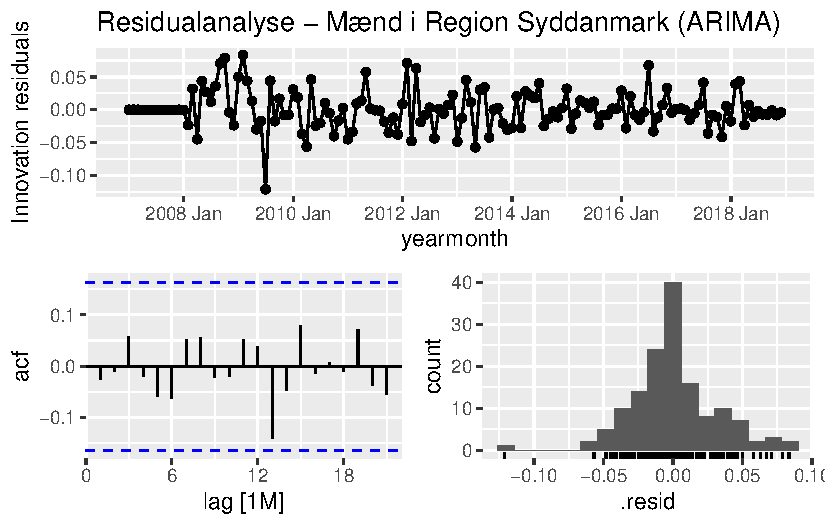
\includegraphics[keepaspectratio]{130625_Forecasting_files/figure-pdf/unnamed-chunk-7-1.pdf}}

Der er kigget nærmere på tidsserien for mænd i region Syddanmark, da den
har relativt høj test-RMSE ift. de andre og høj forskel på trænings- og
testscore.

Residualerne ser ud til at være nogenlunde centreret omkring nul, men
der er enkelte ekstreme udsving (outliers), særligt i 2009 og 2016.

ACF-plottet viser, at der ikke er signifikant autokorrelation i
residualerne --- alle ligger inden for konfidensgrænserne. Det er et
tegn på, at modellen har fanget den systematiske struktur i data.
Histogrammet indikerer en rimelig symmetrisk fordeling, men med lidt
tungere haler end en ideel normalfordeling.

Samlet set tyder residualanalysen på, at modellen er acceptabel, men de
ekstreme observationer og den relativt høje forecastfejl på testdata
(RMSE = 0.085) antyder, at modellen kan være følsom over for enkelte
udsving.

\pandocbounded{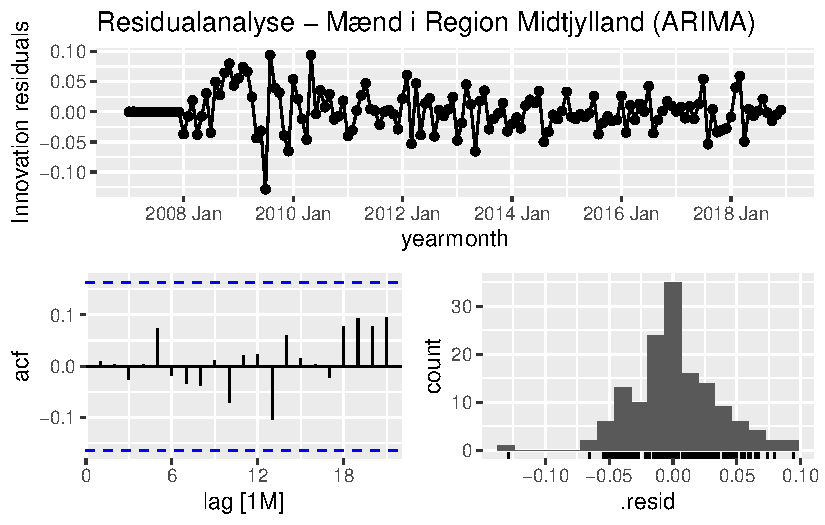
\includegraphics[keepaspectratio]{130625_Forecasting_files/figure-pdf/unnamed-chunk-8-1.pdf}}

Der er kigget nærmere på tidsserien for mænd i region Midtjylland, da
den har lav test-RMSE ift. trænings-RMSE.

Modellen ser ud til at have fanget strukturen i data rimeligt godt.
Residualerne er generelt centreret omkring nul, men enkelte større
afvigelser ses tidligt i serien.

ACF-plottet viser svag autokorrelation ved nogle højere lags, men ingen
værdier ligger tydeligt uden for konfidensgrænserne. Histogrammet viser
en nogenlunde symmetrisk fordeling med lette afvigelser fra normalitet.

Samlet set er der ikke tegn på systematiske fejl i residualerne. Det
stemmer godt overens med den relativt lave RMSE på testdata (RMSE =
0.019) sammenlignet med en højere træningsfejl (RMSE = 0.050), hvilket
tyder på, at modellen generaliserer bedre end forventet.

\pandocbounded{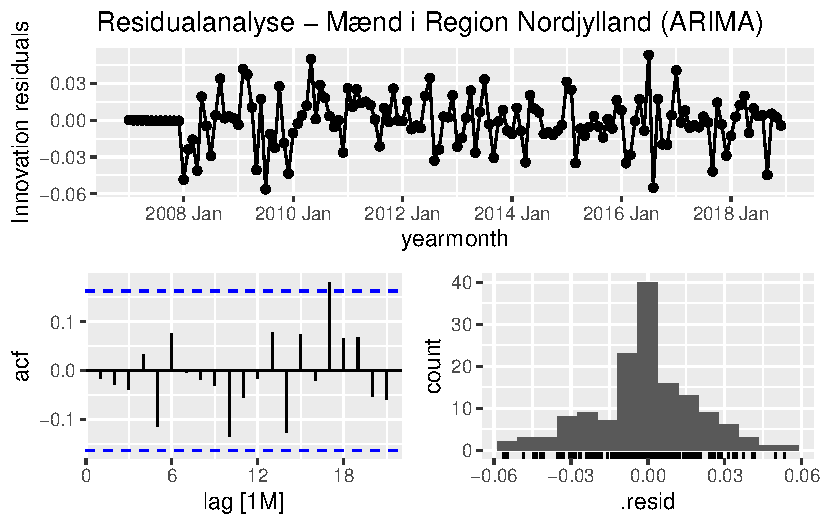
\includegraphics[keepaspectratio]{130625_Forecasting_files/figure-pdf/unnamed-chunk-9-1.pdf}}

Til sidst er der kigget nærmere på tidsserien for kvinder i region
Nordjylland, da den har lav test-RMSE og lav trænings-RMSE.

Residualerne er pænt centreret omkring nul og uden tydelige mønstre over
tid. Der ses enkelte udsving, men ingen systematiske afvigelser.

ACF-plottet viser lidt autokorrelation ved lag 17, men det virker
rimelig tilfældigt og ellers ligger værdierne inden for
konfidensgrænserne, hvilket tyder på, at modellen har fanget den
væsentlige struktur i data. Histogrammet viser en forholsvist symmetrisk
fordeling af residualerne.

Samlet set understøtter residualanalysen, at modellen er velfungerende
for denne serie. Det stemmer overens med en lav forecastfejl på testdata
(RMSE = 0.012) og indikerer, at modellen generaliserer stabilt.

\subsubsection{Ljung-tests for
tidsserier}\label{ljung-tests-for-tidsserier}

For at vurdere, om modellerne har fanget den systematiske struktur i
data, er der udført en Ljung-Box test på residualerne fra hver
vinder-model. Testen er sat op med 24 lags og 3 frihedsgrader og udføres
med features(.innov, ljung\_box).

Resultaterne viser, at 9 ud af 10 modeller har høje p-værdier, hvilket
betyder, at vi ikke forkaster nulhypotesen om uafhængige residualer. Det
tyder på, at modellerne har fanget den væsentlige struktur i data.

Dog er der en klar undtagelse: ETS-modellen for kvinder i Region
Hovedstaden har en meget lav p-værdi, hvilket tyder på signifikant
autokorrelation i residualerne. Det skaber tvivl om modellens gyldighed
her og kunne indikere, at ARIMA muligvis havde været et bedre valg for
denne serie.

Samlet set tyder resultaterne på, at residualerne fra de fleste modeller
kan betragtes som hvid støj, hvilket er et centralt krav i vurderingen
af en god tidsseriemodel.

\section{Sammenligning af 2019 forudsigelser og
virkeligheden}\label{sammenligning-af-2019-forudsigelser-og-virkeligheden}

Plottet nedenfor viser en sammenligning mellem de faktiske observationer
(sort) og modellernes punktprognoser (blå) for 2019, opdelt på køn og
region. Generelt følger prognoserne udviklingen i de faktiske data tæt,
hvilket bekræfter, at modellerne har god forudsigelsesevne.

Særligt for mænd i Region Midtjylland og Nordjylland er der meget tæt
overensstemmelse. Derimod ses systematiske afvigelser for mænd i Region
Syddanmark og kvinder i Region Hovedstaden, hvor modellerne
undervurderer eller overvurderer udviklingen. Det stemmer overens med de
højere RMSE-værdier og residualanalyser for disse serier.

\pandocbounded{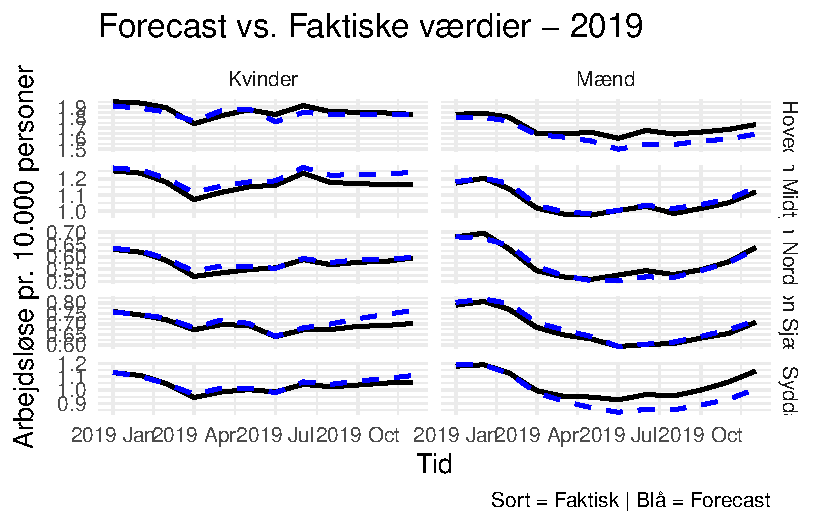
\includegraphics[keepaspectratio]{130625_Forecasting_files/figure-pdf/unnamed-chunk-11-1.pdf}}

\section{Forecasting af 2020 for alle
tidsserier}\label{forecasting-af-2020-for-alle-tidsserier}

Plottet nedenfor viser en 12-måneders fremskrivning af arbejdsløsheden i
2020 baseret på den model, der tidligere blev vurderet som bedst for
hver kombination af køn og region. Forecastet er suppleret med 80\% og
95\% prædiktionsintervaller.

For hovedparten af serierne er ARIMA-modellen anvendt (vist i rød), mens
ETS-modellen (turkis) kun er valgt for kvinder i Region Hovedstaden.

Prognoserne viser overvejende stabile niveauer gennem året, men særligt
for mænd i Region Midtjylland og Region Syddanmark ses en markant
stigning i arbejdsløsheden og bredere prædiktionsintervaller mod årets
slutning. Dette afspejler større usikkerhed i netop disse serier.

Visualiseringen tydeliggør forskellene mellem køn og region og
bekræfter, at modellerne formår at fange både strukturelle niveauer og
variabilitet i data.

\pandocbounded{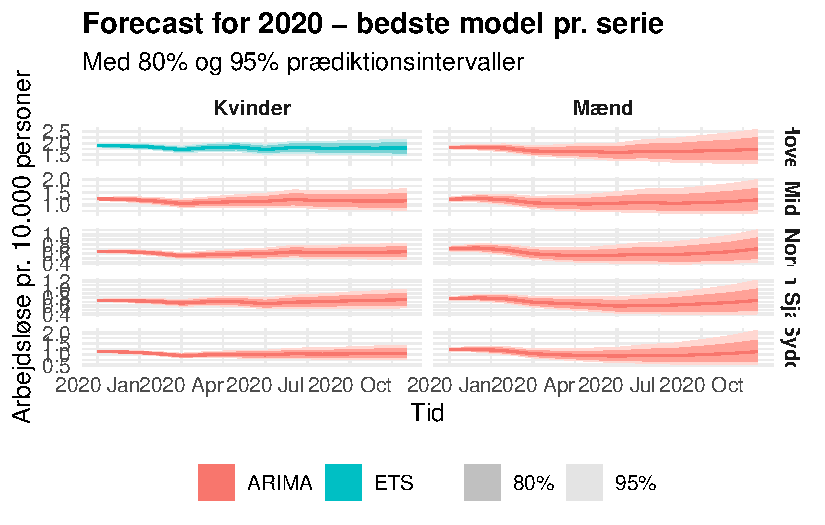
\includegraphics[keepaspectratio]{130625_Forecasting_files/figure-pdf/unnamed-chunk-12-1.pdf}}

Dermed afsluttes forecastdelen med en samlet visualisering, som
underbygger analysens centrale fund og danner baggrund for den
afsluttende vurdering.

\section{Konsklusion}\label{konsklusion}

Denne opgave har undersøgt, hvordan klassiske tidsseriemodeller som
ARIMA, ETS og benchmarkmodellen SNaive kan anvendes til at analysere og
forudsige udviklingen i arbejdsløsheden i Danmark, opdelt på region og
køn. Analysen bygger på ti tidsserier, som dækker perioden 2007 til
2019, og er gennemført med fokus på datamønstre, modelestimering og
forudsigelsespræcision.

Den eksplorative analyse viste tydelige sæsonvariationer og regionale
forskelle i arbejdsløsheden, især blandt mænd. Med log-transformerede
data og STL-dekomposition blev det muligt at fremhæve og vurdere trends
og sæsonkomponenter i de enkelte serier. Beregningen af features og
deskriptive mål bekræftede høj autokorrelation og gennemgående trends,
hvilket er væsentligt for valg af modeltype.

Modelvalideringen pegede på ARIMA som den mest præcise model i ni ud af
ti serier. Krydsvalidering, residualanalyse og Ljung-Box-tests
indikerede generelt, at modellerne var godt tilpasset og havde
uafhængige fejlled. En undtagelse blev identificeret for ETS-modellen i
Region Hovedstaden, hvor residualerne udviste autokorrelation, hvilket
giver anledning til tvivl om modellens egnethed i denne sammenhæng.

Sammenligningen mellem modellernes forudsigelser og de faktiske
observationer i 2019 viste overordnet god overensstemmelse. Prognoserne
for 2020 antyder overvejende stabile niveauer, men med stigende
usikkerhed i visse mandlige serier, særligt i Region Syddanmark og
Midtjylland.

Samlet set viser analysen, at klassiske tidsseriemodeller, særligt
ARIMA, egner sig godt til at beskrive og forudsige arbejdsløsheden i et
dansk kontekstuelt rum, forudsat at modellerne valideres grundigt og
vurderes kritisk i forhold til residualstruktur og prognoseegenskaber.

\newpage

\section{Kildeliste}\label{kildeliste}

Hyndman, R. J., \& Athanasopoulos, G. (2021). Forecasting: principles
and practice (3rd ed.). OTexts. https://otexts.com/fpp3/

OpenAI. (2025). ChatGPT (v.4o) {[}Large language model{]}.
https://chat.openai.com/

\newpage

\section{Bilagsoversigt}\label{bilagsoversigt}

\begin{itemize}
\tightlist
\item
  Bilag 1: Features
\end{itemize}




\end{document}
